\thispagestyle{empty}
\begin{center}
%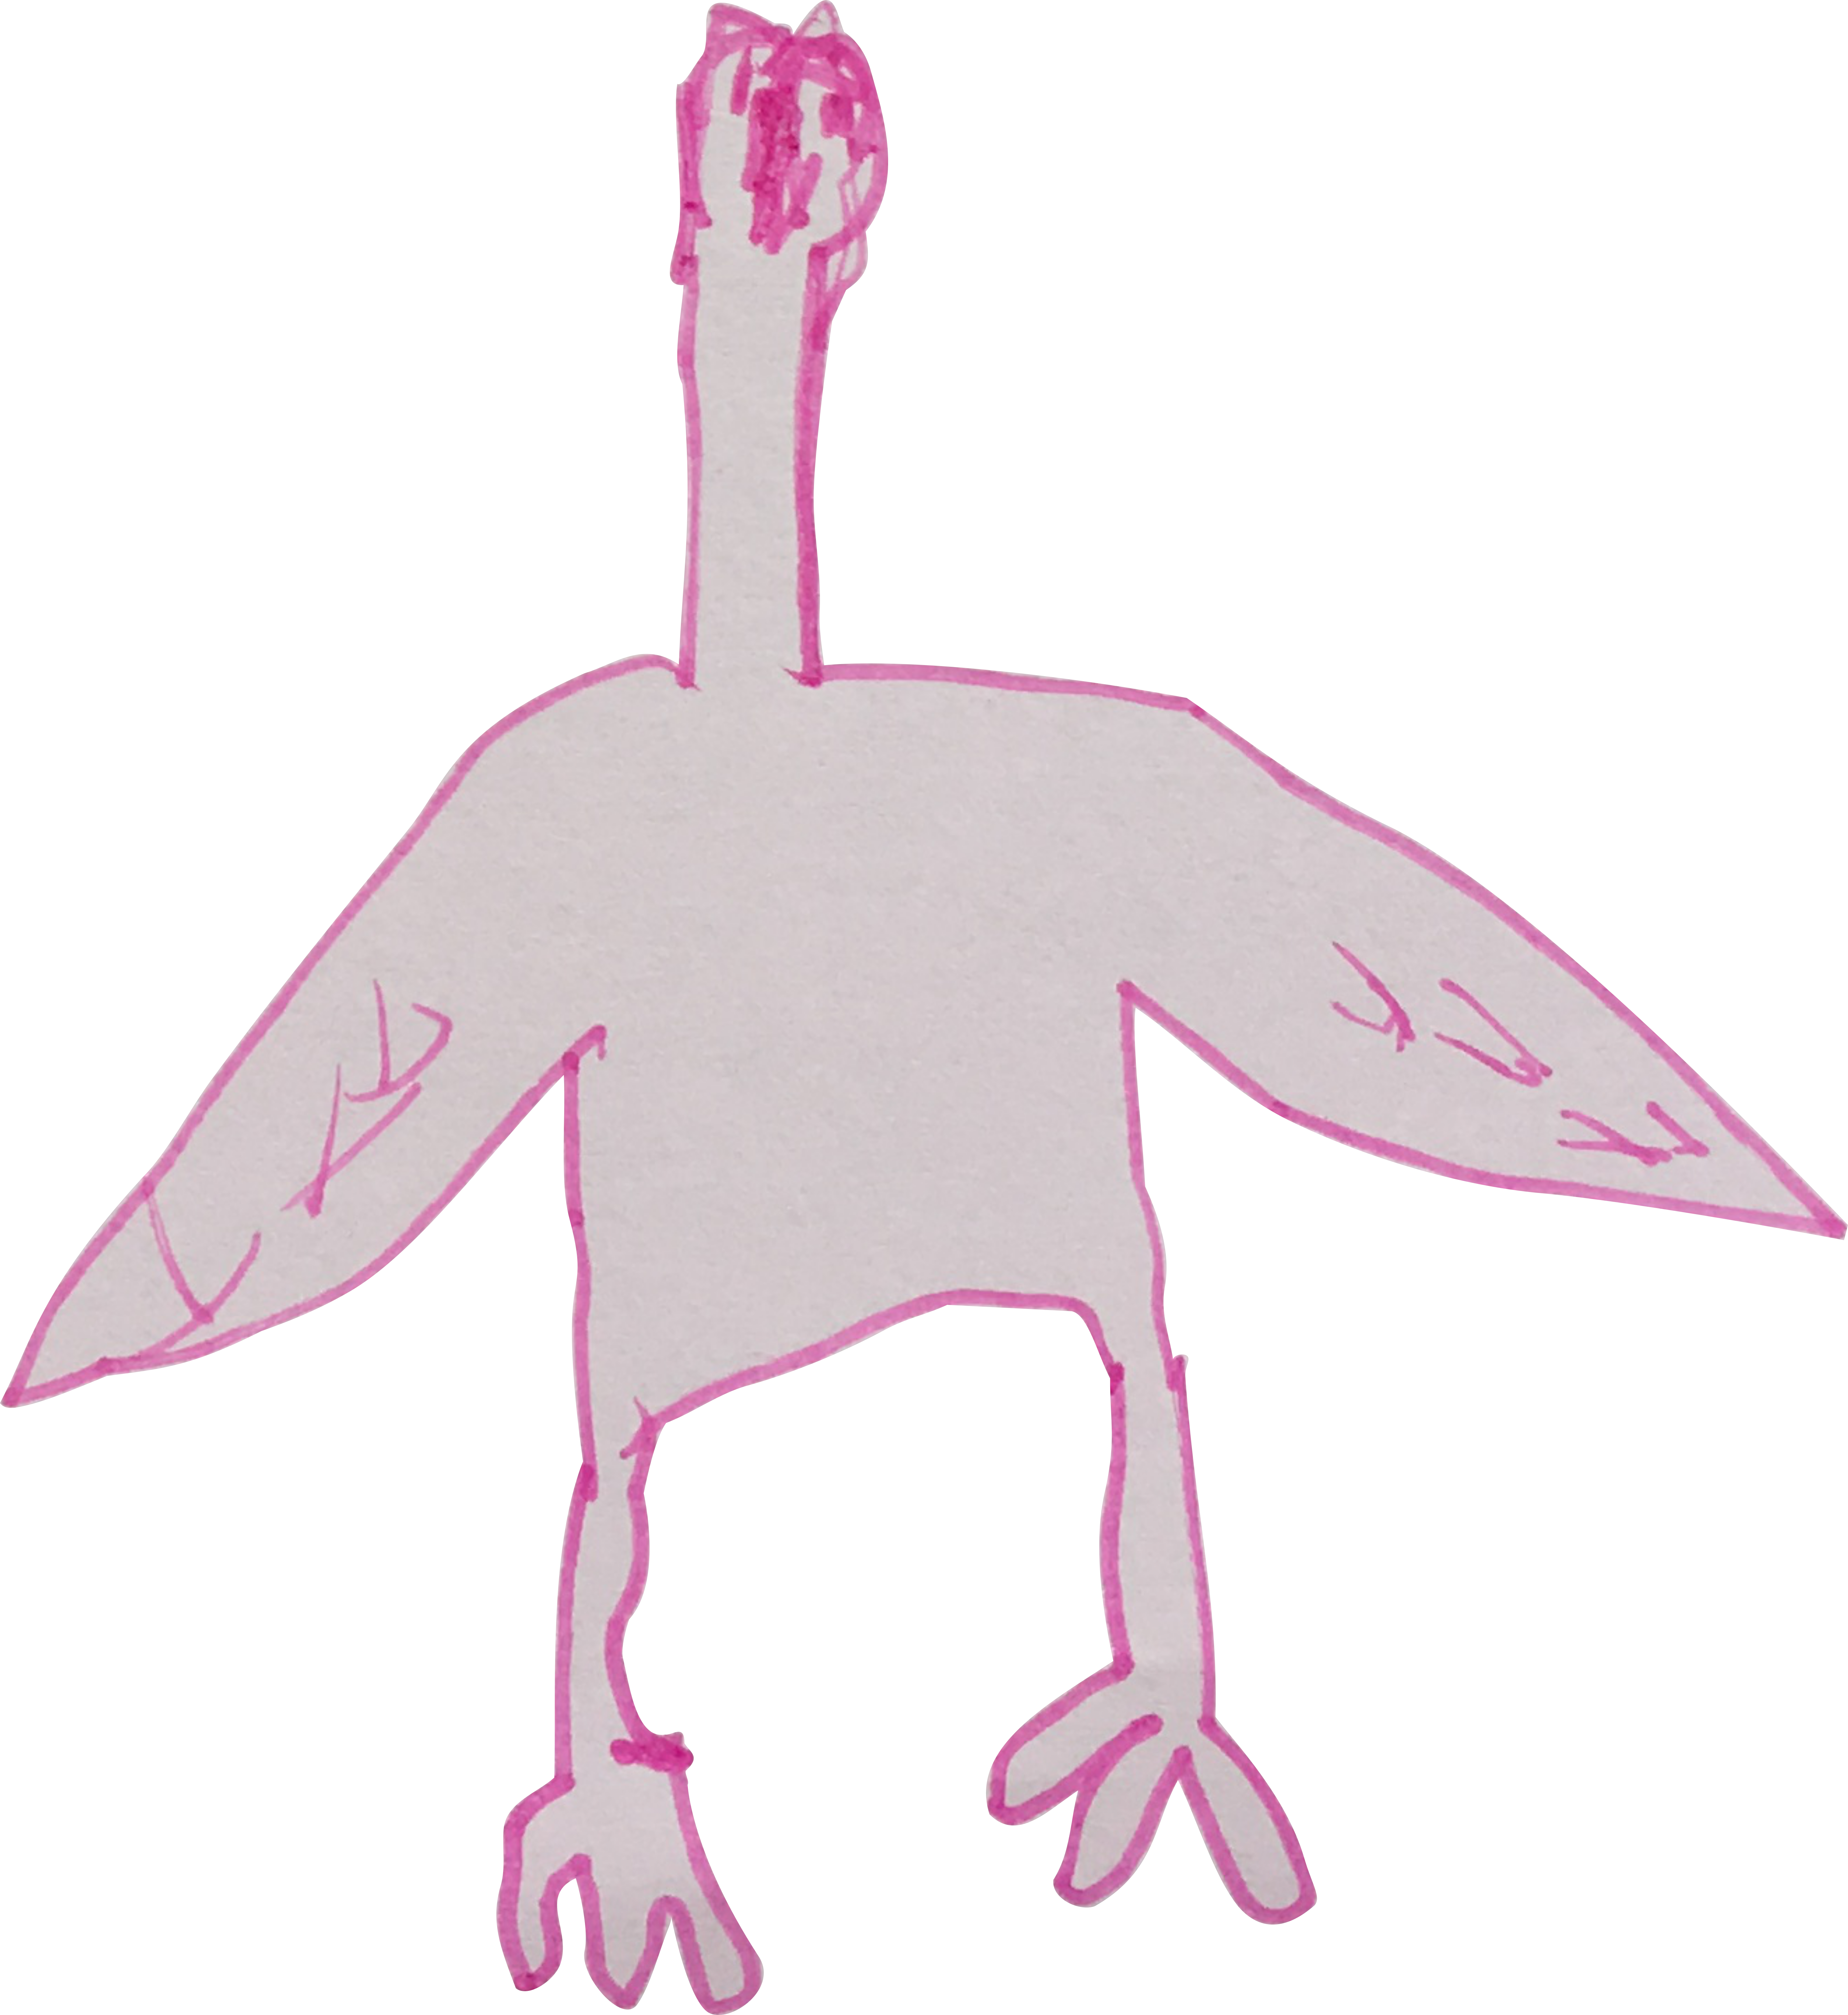
\includegraphics[height=.7\textheight]{./bilder/huhn2.png}
\end{center}
\vskip 2cm
{\Huge\color{farbe}\hfill{\tt{Leo}}}
\addcontentsline{toc}{chapter}{Leo}
\newpage
%%%%%%%%%%%%%%%%%%%%%%%%%%%%%%%%%%%%%%%%%%%%%%%%%%%%%%%%%%%%%%%%%%%%%%%%%%%%%%%
\lettrine[lines=2, lhang=.2, loversize=.25, lraise=0.05, findent=0.1em,
nindent=0em]{{\textooquote}A}{}lle Kinder anziehen bitte! Wir gehen jetzt raus und spielen Schatzsuche.\textcoquote Aysel Ocak aus dem Kindergarten hat Geburtstag. Elin ist auch eingeladen, aber sie kennt hier niemanden. Alles nur Cousins und Cousinen von Aysel, die sich auf Kurdisch unterhalten, und das kann Elin nicht so gut. Papa will zwar immer mit ihr üben, aber sie kann sich einfach nichts merken. Frau Ocak spricht nur wegen ihr Deutsch mit allen.

Und jetzt Schatzsuche. Alle rufen wild durcheinander und Frau Ocak kommt gar nicht hinterher, alle Schuhe zu binden. Eilen ist die letzte, die dran kommt. Da hat ihr Papa wohl doch Recht gehabt, hätte sie mal lieber Kurdisch mit ihm geübt.

Als sie endlich auch fertig ist, sind die anderen Kinder schon mit dem Lift die sieben Stockwerke nach unten gefahren und zum kleinen Wäldchen gelaufen. Frau Ocak versucht zwar zu rufen, die Kinder sollen mal nach Hinweisen suchen, aber der Schatz ist bereits entdeckt. In einem hohlen Baum, da hätte Eilen auch als erstes nachgesehen. 

Wenn man kein Wort versteht, ist man schnell alleine, das merkt Eilen jetzt. Sie beschliesst, selbst noch nach Hinweisen zu suchen. Im Wäldchen kennt sie sich gut aus, hier spielt sie selber auch oft. 

Sie findet einen grossen Luftballon mit einem Pfeil darauf. Der hat sich allerdings so in einem Baum verfangen, dass er sich durch den Wind in alle Richtungen dreht. Eilen wartet, bis der Pfeil auch einmal in die Richtung zeigt, in der sie am liebsten weiter suchen will und geht dann los.

Plötzlich kracht und zischt es ganz gewaltig direkt vor ihr. Äste brechen , die Vögel fliegend aufgeregt davon. Eilen rennt davon, bleibt aber schon nach dem ersten Sprung mit den Haaren in einem Gebüsch hängen. Als sie versucht sich zu befreien, hört sie einen sehr eigenartigen Laut. Sie weiss zwar nicht, von welchem Tier das ist, aber es klingt in ihren Ohren wie ein Hilfeschrei. Da hat sich jemand weh getan, denkt Eilen, überwindet ihre Angst und geht in die Richtung des Geräusches, also da hin, wo eben noch der laute Krach gewesen ist.

Eilen sieht: nichts. Nur der Wald genau so wie er immer ist, nirgends scheint etwas anders zu sein als sonst. Komisch, staunt Eilen. Aber dann hört sie das Wimmern wieder. Viel leiser als vorhin, ganz in ihrer Nähe. Sie sieht sich um und sieht: einen Hund. Aber keinen echten, sondern aus Plüsch. 

Ob der das wohl gewesen ist? Nein, das ist ganz und gar unmöglich. 

\enquote{Da bist du ja!} Frau Ocak kämpft sich durch das Dickicht des Wäldchens. \enquote{Dein Eltern sind schon da und warten auf Dich.}

\enquote{Aber da war etwas, haben sie das nicht gehört?} Aber Frau Ocak hat keinen Sinn für Kindergeschichten und ist schon wieder auf dem Weg zurück. Eilen wirft einen letzten Blick zurück und trottet hinterher.

Im Auto auf der Fahrt nach Hause fragt ihre Mama, was das für ein furchtbar schmutziges Ding sei, dass sie da habe und das ihr das nicht in die Wohnung käme. Erst da wird Eilen bewusst, dass sie den Plüschhund immer noch hat. 

Ohne zu überlegen antwortet Eilen, dass dies Leo sei, der wohne jetzt bei ihr. Der Kompromiss nach dem zu erwartenden Streit mit Mama ist, dass Papa den Hund als erstes in die Waschmaschine stecken wird. Wenn er das überlebt und nicht ganz zerfällt, darf er bleiben.

Am Abend kommt Papa mit Leo aus dem Keller. Leo scheint ein Dackel zu sein, aber ganz sicher ist sich niemand. Jedenfalls muss Mama zugeben, dass Leo wirklich sauber zu sein scheint und erteilt die Erlaubnis.

Eilen hat das Gefühl, dass Leo ihr zuzwinkert. Sie nimmt ihn unter den Arm und geht mit ihm in ihr Zimmer, ihn mal richtig zu bürsten.








\vfill
